\subsection{Defining the measure of discriminative capacity of a filter}
\label{sub:fine-entropy}
Entropy of a filter is calculated to measure its discriminative capacity. The use of entropy is motivated by works such as \cite{Breiman}, \cite{AmitGeman}.
For computing the entropy of a filter, we start by collecting filter responses from a set of $N$ images.
Each image, when passed through the CNN produces a $p \times p$ heat map of scores for each filter in a given layer (e.g., $p = 6$ for a conv-5 filter and $p = 1$ for an fc-6 filter).
This heat map is vectorized (\texttt{x(:)} in MATLAB) into a vector of scores of length $p^2$. With each element of this vector we associate the class label of the image. 
Thus, for every image we have a score vector and a label vector of length $p^2$ each.
Next, the score vectors from all $N$ images are concatenated into an $Np^2$-length score vector.
The same is done for the label vectors.

We define the entropy of a filter in the following slightly different three ways:
\subsubsection{Label Entropy}
\label{sub:def-label-ent}
For a given score threshold $\tau$, we define the \emph{class entropy of a filter} to be the entropy of the normalized histogram of class labels that have an associated score $\geq \tau$.
A low class entropy means that at scores above $\tau$, the filter is very class selective.
As this threshold changes, the class entropy traces out a curve which we call the \emph{entropy curve}.
The \emph{area under the entropy curve} (AuE), summarizes the class entropy at all thresholds and is used as a measure of discriminative capacity of the filter. 
The lower the AuE value, the more class selective the filter is.

\subsubsection{Weighted Label Entropy}
\label{sub:def-weighted-label-ent}
While computing the class label histogram, instead of the label count we use the sum of the scores associated with the labels to construct the histogram. (Note: Since we are using outputs of the rectified linear units, all scores are $\geq 0$.)

\subsubsection{Spatial-Max (spMax) Label Entropy}
\label{sub:def-spmax-label-ent}
Instead of vectorizing the heatmap, the filter response obtained as a result of max pooling the $p \times p$ filter output is associated with the class label of each image. Thus, for every image we have a score vector and a class label vector of length $1$ each.
Next, the score vectors from all $N$ images are concatenated into an $N$-length score vector.
Then, we proceed in the same way as for the case of Label-Entropy to compute the AuE of each filter. 

\subsection{Defining the measure of discriminative capacity of a layer}
The discriminative capacity of layer is computed as following: The filters are sorted in increasing order of their AuE.
Next, the cumulative sum of AuE values in this sorted list is calculated. The obtained list of Cumulative AuEs is referred to as CAuE. 
Note that, the $i$-th entry of the CAuE list is the sum of the AuE scores of the top $i$ most discriminative filters.
The difference in the value of the $i$-th entry before and after fine-tuning measures the change in class selectivity of the top $i$ most discriminative filters due to fine-tuning.
For comparing results across different layers, the CAuE values are normalized to account for different numbers of filters in each layer. 
Specifically, the $i$-th entry of the CAuE list is divided by $i$. 
This normalized CAuE is called the Mean Cumulative Area Under the Entropy Curve (MCAuE).
A lower value of MCAuE indicates that the individual filters of the layer are more discriminative.

\setlength{\tabcolsep}{1pt}
\begin{table}
\begin{center}
\caption{This table lists percentage decrease in MCAuE as a result of finetuning when only 0.1, 0.25, 0.50 and 1.00 fraction of all the filters were used for computing MCAuE. A lower MCAuE indicates that filters in a layer are more selective/class specific. The 0.1 fraction includes the top 10\% most selective filters, 0.25 is top 25\% of most selective filters. Consequently, comparing MCAuE at different fraction of filters gives a better sense of how selective the ``most" selective filters have become.
A negative value in the table below indicates increase in entropy. Note that for all the metrics maximum decrease in entropy takes place while moving from layer 5 to layer 7. Also, note that for fc-6 and fc-7 the values in Label-Entropy and spMax-Label-Entropy are same as these layers have spatial maps of size 1.}
\label{table:fine-change}
\scalebox{0.85}{
\newcolumntype{d}[2]{D{.}{\cdot}{#1} }
\begin{tabular}{|c|p{1cm} p{1cm} p{1cm} p{1cm}| p{1cm} p{1cm} p{1cm} p{1cm}|p{1cm} p{1cm} p{1cm} p{1cm}|}
\hline
Layer & \multicolumn{4}{c|}{Label-Entropy} & \multicolumn{4}{c|}{Weighted-Label-Entropy} & \multicolumn{4}{c|}{spMax-Label-Entropy} \\
\hline
& 0.1 & 0.25 & 0.5 & 1.0 & 0.1 & 0.25 & 0.5 & 1 & 0.1 & 0.25 & 0.5 & 1.0 \\
\hline
conv-1 & $-0.02$  & $-0.14 $  & $-0.19$  & $-0.19$  & $0.06$  & $-0.13$  & $-0.16$  & $-0.16$  & $0.19$  & $0.10$  & $0.07$  & $0.04$   \\
conv-2 & $-0.71$  & $-0.31$   & $-0.14$  & $0.01$  & $0.41$  & $0.53$  & $0.58$  & $0.57$  & $-0.39$  & $-0.03$  & $0.11$  & $0.23$  \\ 
conv-3 & $-1.14$  & $-0.86$   & $-0.67$  & $-0.44$ & $1.11$  & $0.66$  & $0.52$  & $0.32$ & $0.14$  & $0.20$  & $0.32$  & $0.33$   \\
conv-4 & $-0.54$  & $-0.31$  & $-0.19$  & $-0.05$ & $-0.10$  & $0.55$  & $0.64$  & $0.57$  & $0.93$  & $0.97$  & $0.80$  & $0.65$ \\
conv-5 & $0.97$  & $0.55$  & $0.43$  & $0.36$ & $5.84$  & $3.53$  & $2.66$  & $1.85$  & $4.87$  & $3.05$  & $2.31$  & $1.62$   \\
fc-6 & $6.52$  & $5.06$  & $3.92$  & $2.64$  & $9.59$  & $7.55$  & $6.08$  & $4.27$ & $6.52$  & $5.06$  & $3.92$  & $2.64$   \\
fc-7 & $5.17$  & $2.66$  & $1.33$  & $0.44$  & $20.58$  & $14.75$  & $11.12$  & $7.78$  & $5.17$  & $2.66$  & $1.33$  & $0.44$  \\
\hline
\end{tabular}}
\end{center}
\end{table}
\setlength{\tabcolsep}{1.4pt}

\begin{figure}[t!]
\centering
\subfloat[Weighted Label Entropy]{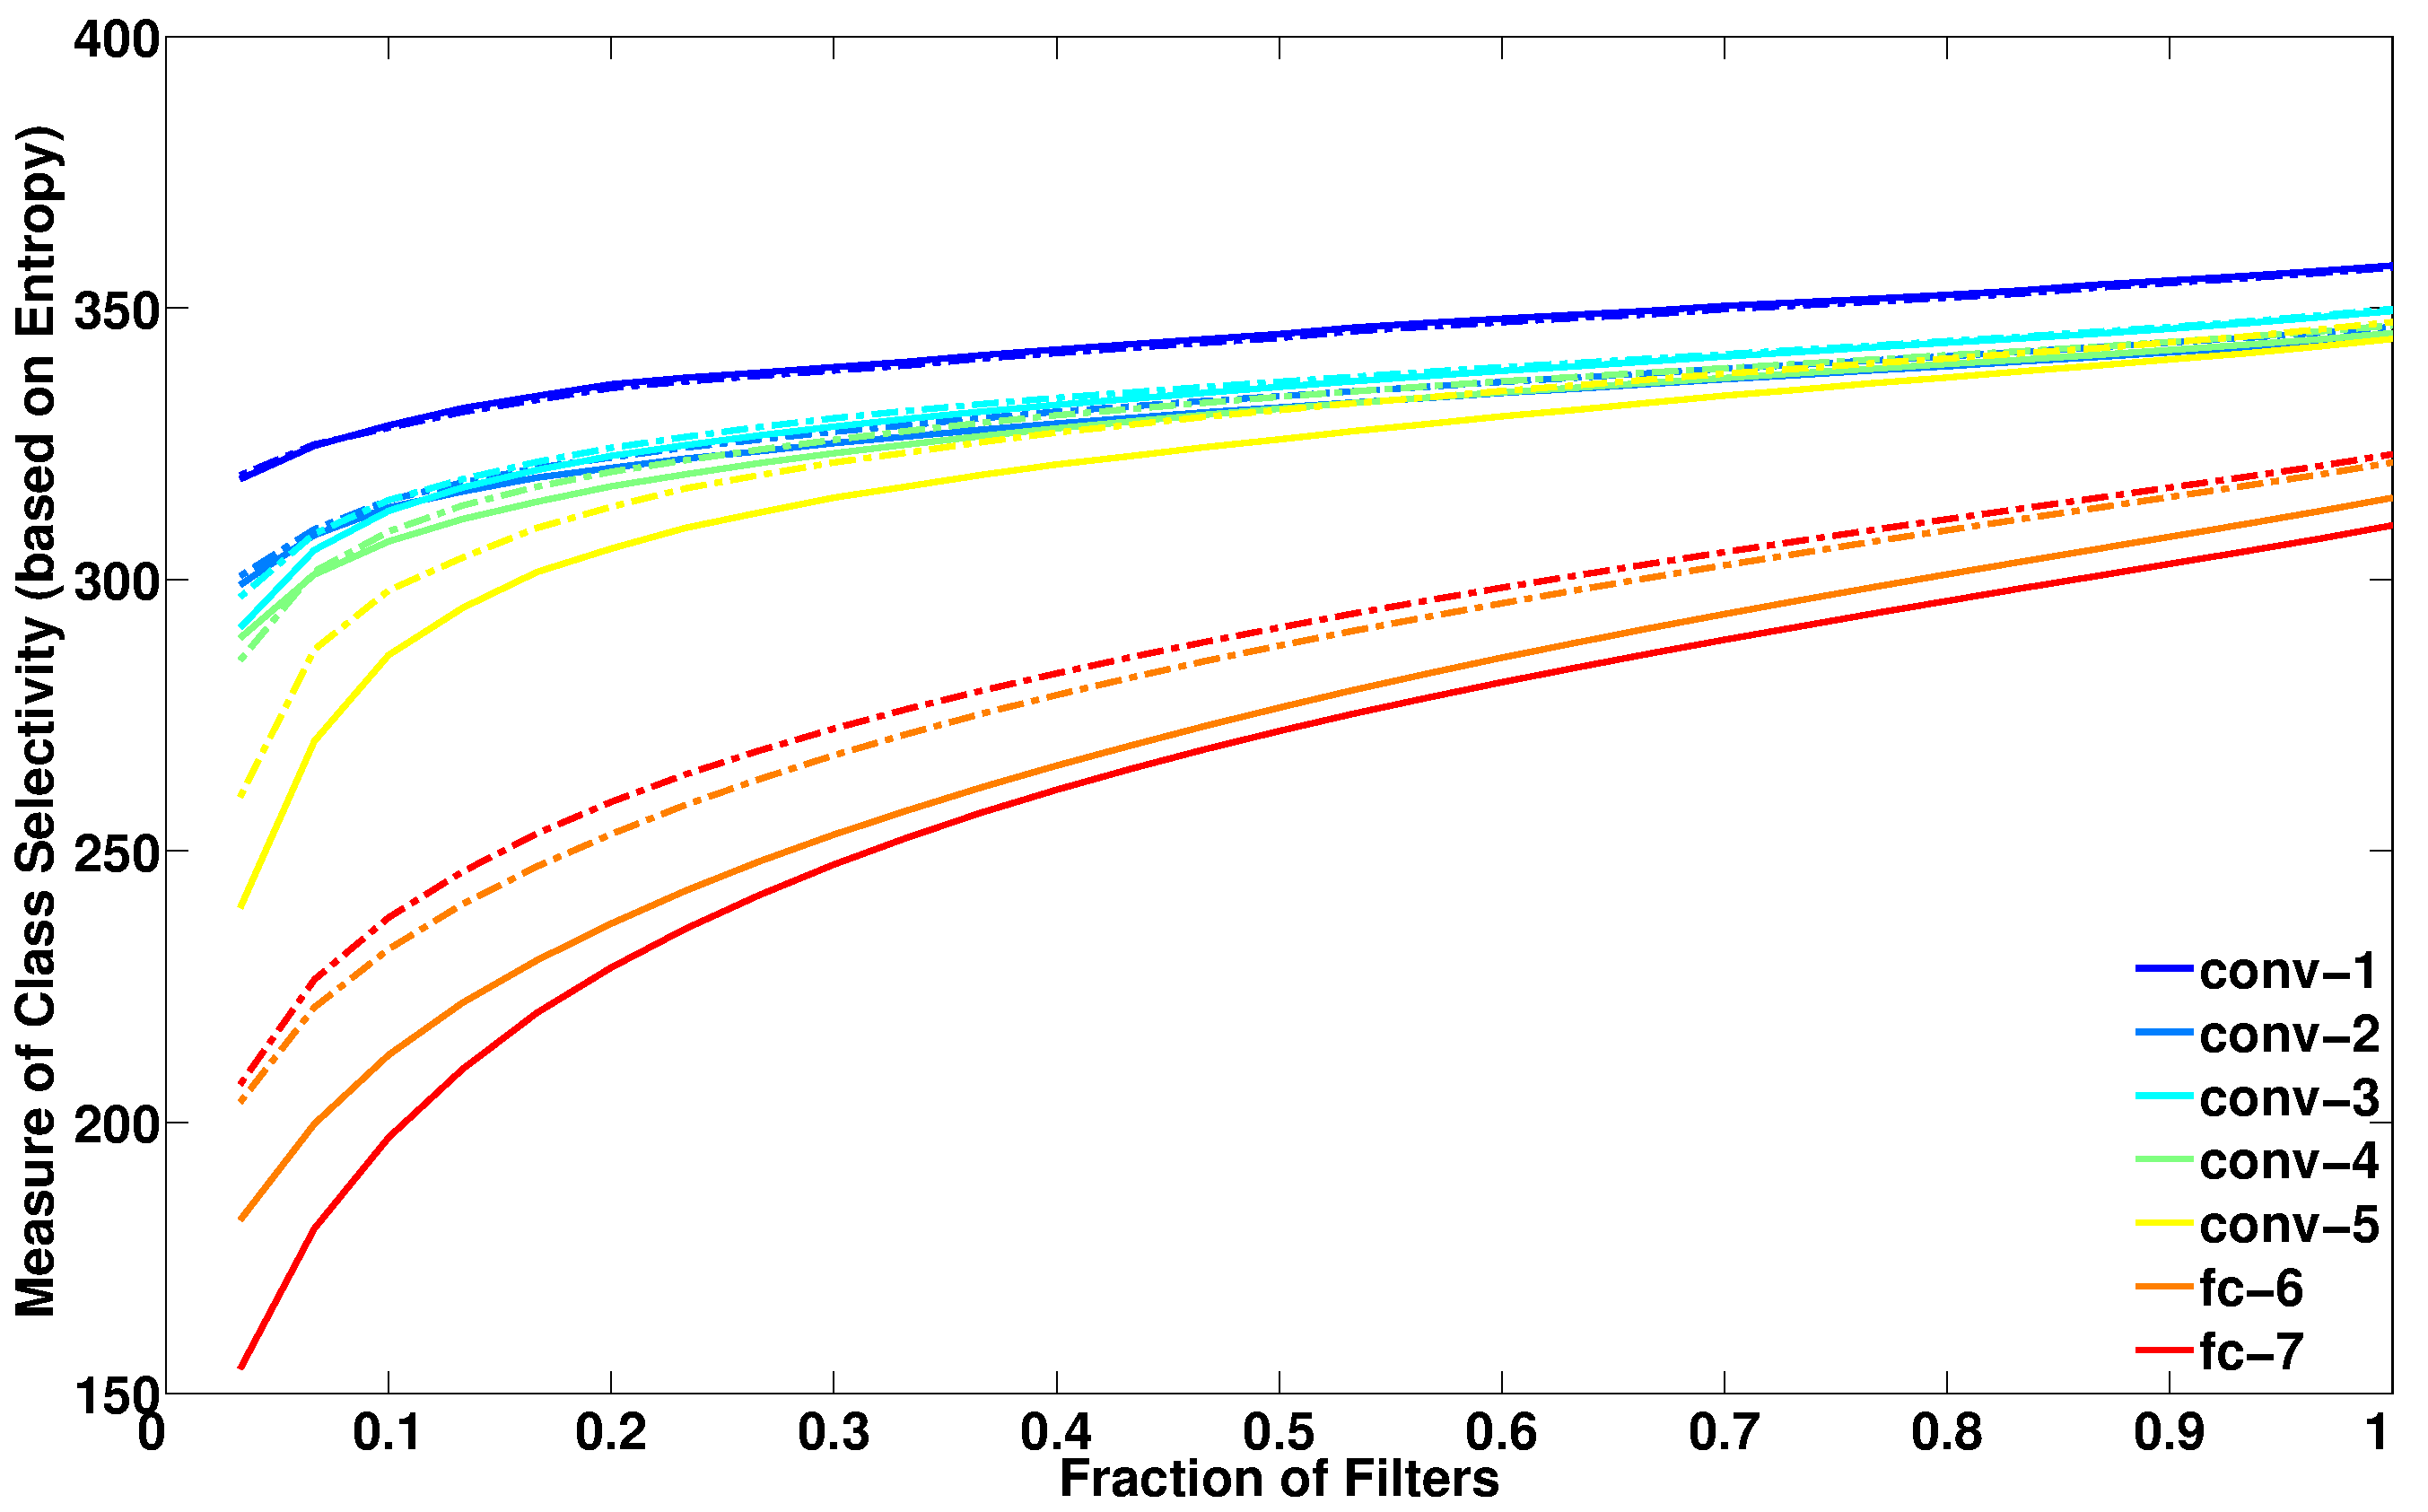
\includegraphics[width=0.95\linewidth]{images/MCAUE_weights.pdf}} \\
\subfloat[Spatial-Max Label Entropy]{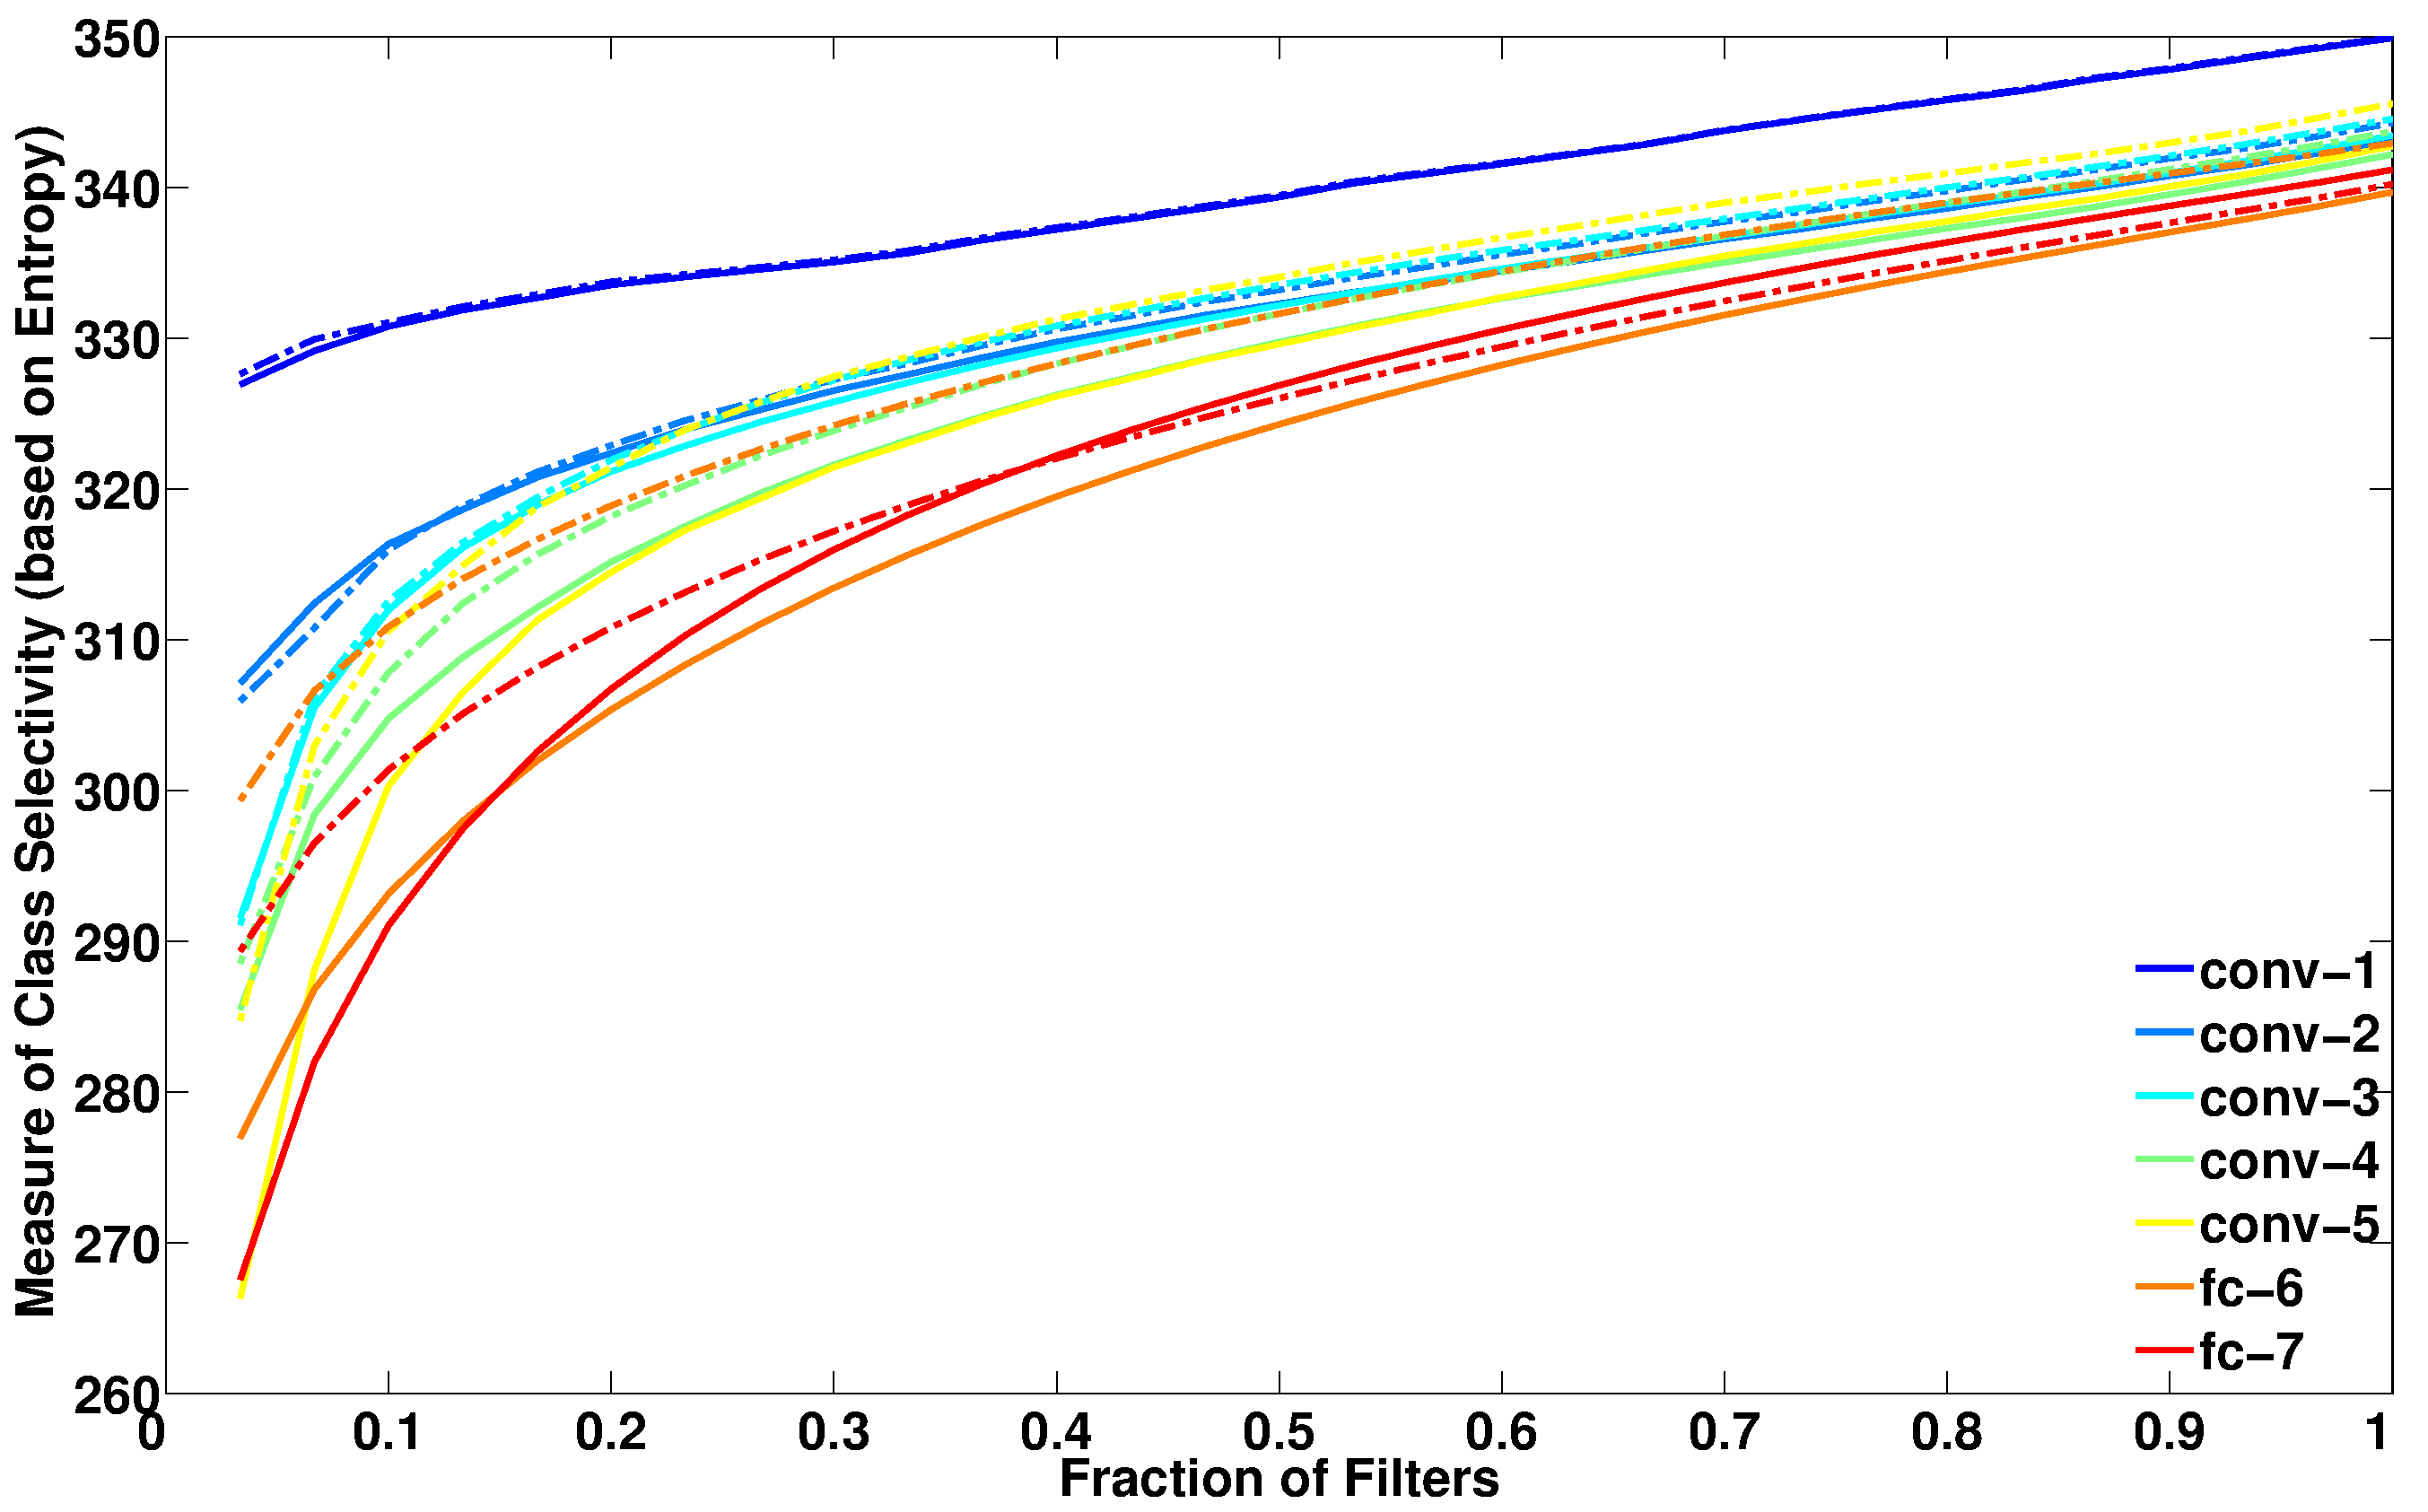
\includegraphics[width=0.95\linewidth]{images/MCAUE_spMax.pdf}}
\caption{PASCAL object class selectivity (measured as MCAuE) plotted against the fraction of filters, for each layer, before fine-tuning (dash-dot line) and after fine-tuning (solid line). A lower value indicates greater class selectivity. (a),(b) show MCAUE computed using Weighted-Label-Entropy and Spatial-Max Label-Entropy method respectively.}
\label{fig:fine-entropy}
\end{figure}

\subsection{Discussion}
The MCAuE measure of determining layer selectivity before and after fine-tuning is shown in figure \ref{fig:fine-entropy} for Weighted Label and Spatial-Max Label entropy. Results for Label entropy method are presented in the main paper. A quantitative measure of change in entropy due to finetuning, computed as percentage change is defined as following:
\begin{eqnarray}
\text{Percent Decrease} = 100 \times \frac{MCAuE_{pre} - MCAuE_{fine}}{MCAuE_{pre}}
\end{eqnarray}
where, $MCAuE_{fine}$ is for fine-tuned network and $MCAuE_{untuned}$ is for network trained on imagenet only. The results are summarized in table \ref{table:fine-change}.
 
As measured by Label entropy layers 1 to 5, undergo negligible change in their discriminative capacity, whereas layers 6-7 become a lot more discriminative. Whereas, the measures of Weighted Label and Spatial-Max Label entropy indicate that only layers 1 to 4 undergo minimal changes and other layers become substantially more discriminative. These results confirm the intuition that lower layers of the CNN are more generic features, whereas fine-tuning mostly effects the top layers. Also, note that these results are true for fine-tuning for moderate amount of training data available as part of PASCAL-DET. It is yet to be determined how lower convolutional layers would change due to fine-tuning when more training data is available. 